\documentclass[9pt,oneside]{book}

\usepackage{xcolor}
\usepackage{mathtools}
\usepackage[legalpaper, margin=0.5in]{geometry}
\usepackage{amsmath}
\usepackage{amssymb}
\usepackage{paralist}
\usepackage{rsfso}
\usepackage{amsthm}
\usepackage[inline]{enumitem}   
\usepackage{lipsum}

\newtheoremstyle{break}
  {\topsep}{\topsep}%
  {\itshape}{}%
  {\bfseries}{}%
  {\newline}{}%
\theoremstyle{break}
\theoremstyle{break}
\newtheorem{axiom}{Axiom}
\newtheorem{thm}{Theorem}[section]
\newtheorem{lem}{Lemma}[thm]
\newtheorem{prop}[lem]{Proposition}
\newtheorem{corL}{Corollary}[lem]
\newtheorem{corT}[lem]{Corollary}
\newtheorem{defn}{Definition}[corL]

\newcommand{\R}{\mathbb{R}}
\newcommand{\N}{\mathbb{N}}
\newcommand{\Z}{\mathbb{Z}}
\newcommand{\Q}{\mathbb{Q}}
\newcommand{\A}{\mathcal{A}}
\newcommand{\J}{\mathcal{J}}
\newcommand{\T}{\mathcal{T}}
\newcommand{\C}{\mathcal{C}}
\newcommand{\M}{\mathcal{M}}
\newcommand{\Complex}{\mathbb{C}}
\newcommand{\Power}{\mathcal{P}}
\newcommand{\pd}{\partial}
\newcommand{\ee}[1]{\cdot 10^{#1}}
\newcommand{\ihat}{\hat{\i}}
\newcommand{\jhat}{\hat{\j}}
\newcommand{\khat}{\hat{k}}



\newcommand{\note}{\color{red}Note: \color{black}}
\newcommand{\remark}{\color{blue}Remark: \color{black}}
\newcommand{\example}{\color{green}Example: \color{black}}
\newcommand{\exercise}{\color{green}Exercise: \color{black}}



\newcommand\blfootnote[1]{%
  \begingroup
  \renewcommand\thefootnote{}\footnote{#1}%
  \addtocounter{footnote}{-1}%
  \endgroup
}

\makeatletter
\def\@seccntformat#1{%
  \expandafter\ifx\csname c@#1\endcsname\c@section\else
  \csname the#1\endcsname\quad
  \fi}
\makeatother

\makeatletter
\newcommand*{\rom}[1]{\expandafter\@slowromancap\romannumeral #1@}
\makeatother

\makeatletter
% This command ignores the optional argument for itemize and enumerate lists
\newcommand{\inlineitem}[1][]{%
\ifnum\enit@type=\tw@
    {\descriptionlabel{#1}}
  \hspace{\labelsep}%
\else
  \ifnum\enit@type=\z@
       \refstepcounter{\@listctr}\fi
    \quad\@itemlabel\hspace{\labelsep}%
\fi}
\makeatother
\parindent=0pt


\begin{document}
\blfootnote{Jinyan Miao; Winter 2022; CC BY-NC-SA; University of Michigan; Physics 401; Professor Bing Zhou}
$$\vec{p} = m\vec{v}\qquad \vec{v} = \vec{\omega}\times \vec{r} \qquad \vec{L} = I\vec{\omega} = \vec{r}\times \vec{p}\qquad \vec{N} = \frac{d\vec{l}}{dt}=\vec{r}\times \vec{F}\qquad U = \frac{1}{2}I \omega^2 \qquad I = \int_V r^2\, dm \qquad I = I_{CM} + Ml^2$$

\begin{align*}
dA = (r\,d\theta)(r\sin(\theta)\, d\phi) = r^2 \sin(\theta) \,d\theta\, d\phi \qquad  d\Omega \coloneqq \frac{dA}{r^2} = \sin(\theta) \,d\theta\, d\phi \qquad  d\Omega' = 2\pi \sin(\theta) \,d\theta \qquad \frac{d\sigma}{d\Omega'} \coloneqq \frac{1}{n_b}\frac{dN}{d\Omega'} = \frac{b}{\sin(\theta)}\left|\frac{db}{d\theta}\right|
\end{align*}

Every beam of particle in the annulus defined by $b$ and the $b+|db|$ area is scattered into the solid angle $d\Omega'$, define by $\theta$ and $\theta+d\theta$. Beam intensity $n_b$ is the number of particle per unit area. $N$ is the number of scattered particles. Note here $|\frac{db}{d\theta}|$ is absolute. Positive $db$ may give negative $d\theta$, that is, increase in $b$ might result in decrease in $\theta$ as force become weaker and so we have less scattering. In experiment, we often put our detector in a place with a distance $d$ from the interaction point, and the detector detects a total area $S$, so the solid angle coverage of the detector is given by $\Delta \Omega = \frac{S}{d^2}$. Now we can calculate the cross section $\sigma(\theta)$ if the force law for scattering is given, and we can use $\sigma(\theta)$ to predict the event rate in experiment set up, we get $\sigma(\theta) = \frac{1}{n_b}\frac{dN}{d\Omega'}$ hence $N(\theta) = n_b\cdot \sigma(\theta)\cdot \Delta \Omega$.\\

In rotational frame $S'$, $\vec{\omega}$ is the angular velocity, $\vec{v}'$ is the velocity of the object in $S'$, $\vec{r}$ is the position of the object in $S$. $-2m \vec{\omega}\times \vec{v}'$ is known as the Coriolis force, and $-m\vec{\omega}$ is known as the Centrifugal force. Force acted on particle in $S'$ reads:
\begin{align*}
\vec{F}' = m\vec{a}' = \vec{F} - m \frac{d\vec{\omega}}{dt}\times \vec{r} - m \vec{\omega} \times (\vec{\omega} \times \vec{r}) - 2m \vec{\omega}\times \vec{v}'
\end{align*}

For discrete distribution, $\{a,b,c\} = \{x,y,z\}$.For continuous mass distribution, $\vec{r} = (r_1, r_2, r_3)$. Let $\{i,j,k\} = \{1,2,3\}$.
\begin{align*}
I_{aa} = \sum_i m_i (b_i^2 + c_i^2) \qquad I_{ab} = I_{ba} = -\sum_i m_i a_i b_i \qquad 
I_{ii} = \int (r_j^2 + r_k^2) \, dm \qquad  I_{ij} = -\int r_ir_j\, dm
\end{align*}
Combining, one can show that we have:
\begin{align*}
\vec{L} = \mathbf{I}\cdot \vec{\omega} = \begin{bmatrix}
L_x \\ L_y \\ L_z
\end{bmatrix} = 
\begin{bmatrix}
I_{xx} & I_{xy} & I_{xz} \\
I_{yx} & I_{yy} & I_{yz}\\
I_{zx} & I_{zy} & I_{zz}
\end{bmatrix} 
\begin{bmatrix}
\omega_x \\ 
\omega_y \\
\omega_z
\end{bmatrix} \qquad \qquad
\begin{cases}
N_1 = I_1 \dot{\omega}_1 - (I_2-I_3)\omega_2 \omega_3 \\
N_2 = I_2 \dot{\omega}_2 - (I_3 - I_1) \omega_3 \omega_1 \\
N_3 = I_3 \dot{\omega}_3 - (I_1 - I_2) \omega_1 \omega_2
\end{cases} \qquad \qquad
\begin{cases}
(I_1 - I_3) \omega_2 \omega_3 - I_1 \dot{\omega}_1 = 0 \\
(I_3 - I_1) \omega_3 \omega_1 - I_1\dot{\omega}_2 = 0 \\ 
I_3 \dot{\omega}_3 = 0
\end{cases} 
\end{align*}

\begin{center}
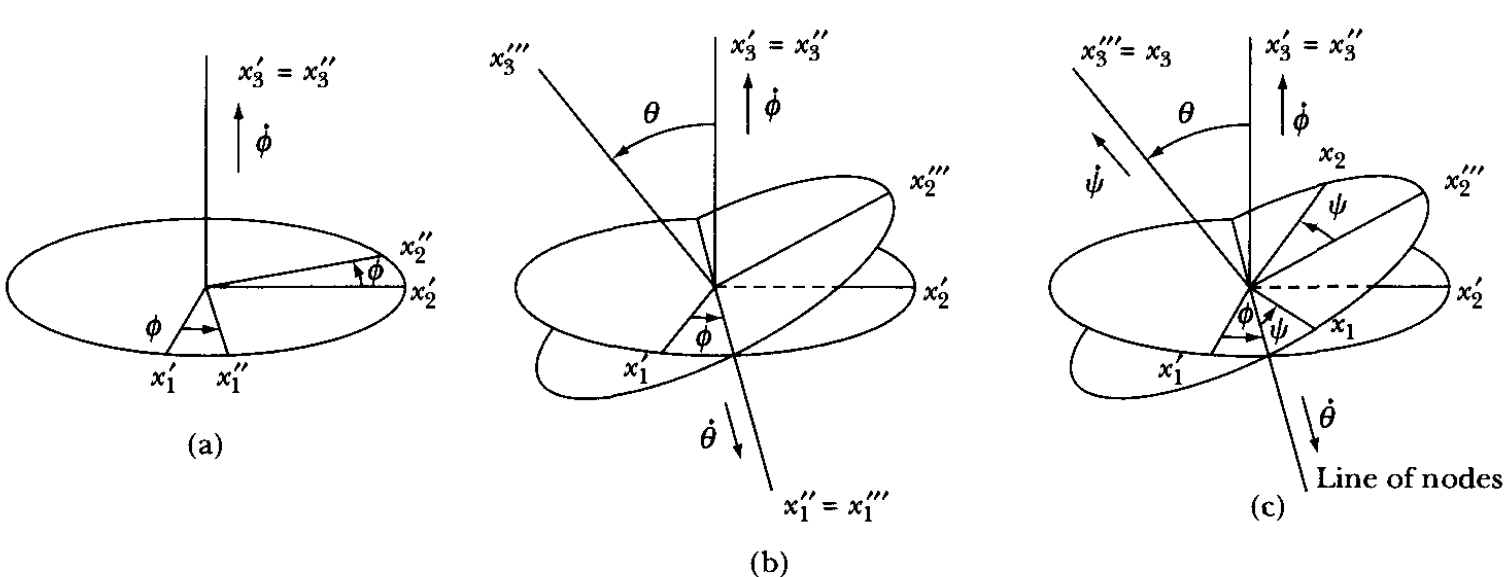
\includegraphics[scale=0.35]{eulerian1.png}
\end{center}

\begin{align*}
\begin{cases}
\dot{\phi}_1 = \dot{\phi} \sin(\theta) \sin(\psi)\\ \dot{\phi}_2 = \dot{\phi} \sin(\theta) \cos(\psi)\\
\dot{\phi}_3 = \dot{\phi}\cos(\theta)
\end{cases}
\qquad\qquad
\begin{cases}\dot{\theta}_1 = \dot{\theta} \cos(\psi) \\
\dot{\theta}_2 = -\dot{\theta}\sin(\psi) \\
\dot{\theta}_3 = 0\\
\end{cases}
\qquad\qquad
\begin{cases}
\dot{\psi}_1 = 0\\
\dot{\psi}_2 = 0\\
\dot{\psi}_3 = \dot{\psi}
\end{cases}\qquad\qquad
\begin{cases}
\omega_1 = \dot{\phi}\sin(\theta)\sin(\psi) + \dot{\theta}\cos(\psi)\\
\omega_2 = \dot{\phi}\sin(\theta) \cos(\psi) - \dot{\theta}\sin(\psi) \\
\omega_3 = \dot{\phi}\cos(\theta) + \dot{\psi}
\end{cases}
\end{align*}



\begin{align*}
\Omega = \frac{I_3 - I_1}{I_1}\, \omega_3 \qquad\qquad
T_{\text{rot}} =  \frac{1}{2}\vec{\omega} \cdot \left(\mathbf{I}\cdot \vec{\omega}\right) &= \frac{1}{2}(\omega_x L_x + \omega_y L_y + \omega_z L_z) 
\end{align*}

Lagrangian for coupled oscillator:
\begin{align*}
\mathcal{L} = T - U = \left( \frac{1}{2}\sum_{j,k}m_{jk}\dot{q}_{j}\dot{q}_k\right) - \left( \frac{1}{2}\sum_{j,k}A_{jk}q_jq_k\right)
\qquad\qquad
\frac{\partial \mathcal{L}}{\partial q_j} - \frac{d}{dt}\frac{\partial \mathcal{L}}{\partial \dot{q}_j} = 0 \qquad \Rightarrow \qquad \frac{\partial U}{\partial q_j} + \frac{d}{dt}\frac{\partial T}{\partial \dot{q}_j} = 0
\end{align*}


\begin{align*}
\det\left(\mathbf{A} - \omega^2 \mathbf{M}\right) = 0  \qquad
q_k(t) = \sum_{r} c_{r}^+ a_{kr} e^{i \omega_r t} + c_\alpha^- a_{kr}e^{-i\omega_r t} \qquad 
\eta_r (t) = c_r^+ e^{i \omega_r t} + c_r^- e^{-i \omega_r t}\qquad
q_k(t) = \sum_r a_{kr}\eta_r(t)
\end{align*}



In summary, when dealing with general coupled oscillations, one wants to find the characteristic frequencies $\omega_r$ to describe the coordinates $\eta_r$ of the normal mode motion. The actual application of the method can be summarized by the followings:
\begin{enumerate}[topsep=3pt,itemsep=-1ex,partopsep=1ex,parsep=1ex]
\item Choose generalized coordinates from the equilibrium of the system.
\item Find kinetic energy $T$ and potential energy $U$ to construct the Lagrangian of the system.
\item Find the matrix $\mathbf{A}$ and matrix $\mathbf{M}$ from the Lagrangian of the system.
\item Determine $\omega_r$ through the secular equation of the system.
\item For each $\omega_r$, find the linear space for the coefficient $\vec{a}_r$ by equation (LSK).
\item Determine the normal coordinates $\eta_r$ with linear combinations of $q_j$ by using equation (NMS). 
\end{enumerate}
\begin{align*}
\mathcal{L} = T - U = \frac{1}{2}\sum_\alpha (\dot{\eta}_\alpha^2 - \omega_\alpha^2 \eta_\alpha^2)
\end{align*}


Small angle approximation:
\begin{align*}
\sin(\theta) \approx \theta \qquad \cos(\theta) \approx 1-\frac{\theta^2}{2} \approx 1 \qquad \tan(\theta) \approx \theta \qquad \cos(\theta_1 - \theta_2) \approx 1
\end{align*}


\end{document}